\documentclass[11pt]{article}
\usepackage[margin=2.5cm]{geometry}
\usepackage{amsmath}\usepackage{amssymb}\usepackage{graphicx}
\usepackage{booktabs}\usepackage{hyperref}
\graphicspath{{../../plots/emulator_tier3/}}
\newcommand{\Mpch}{\,h^{-1}\,\mathrm{Mpc}}
\newcommand{\code}[1]{\texttt{#1}}
\newcommand{\Cemu}{C_{\rm emu}}
\newcommand{\Ccv}{C_{\rm CV}}
\title{The emulator-based Fisher for ASTRA clustering}
\author{ASTRA clustering project}\date{June 2026}
\begin{document}\maketitle

\begin{abstract}
The original ASTRA Fisher forecast had two structural weaknesses: derivatives from
the HOD-mismatched $\pm$ cosmology pairs (HOD contamination -- the Tier-0/1 subtraction
saga), and a covariance $C=C_{\rm CV}$ that implicitly assumes a perfect emulator (which
we showed over-states the ASTRA value-add). The Tier-3 emulator removes both: it gives
\emph{HOD-clean} derivatives $\partial\xi/\partial\theta$ at fixed HOD for the full
$w_0w_a$CDM$+$ parameter set (including $w_0,w_a$), and we have \emph{measured} the
emulator-error covariance $C_{\rm emu}$. This note defines the emulator-based Fisher
($C=C_{\rm CV}+C_{\rm emu}$, joint cosmology$+$HOD with HOD marginalisation), validates
it against the MCMC, and uses it to forecast the campaign payoff. It is the companion to
\code{mlp\_emulator\_note} (which builds the emulator and the inference prototype).
\end{abstract}

\section{Why a new Fisher}
The Fisher matrix is $F_{ab}=\sum (\partial_a\xi)\,C^{-1}\,(\partial_b\xi)$; its quality
is set entirely by the derivatives and the covariance. The original forecast
(\code{notes/fisher}, \code{vector\_search}) had known problems in both:
\begin{itemize}
\item \textbf{Derivatives.} Central differences over the $\pm2$--$3\%$ AbacusSummit
  pairs are \emph{not} HOD-matched, so the HOD mismatch contaminated
  $\partial\xi/\partial\theta$ at a level comparable to the cosmology signal --- worst
  for $\sigma_8$ (the raw derivative was $\sim$11\% of the expected $2\xi$). Tiers 0/1
  fought this with a noise model and an explicit $\partial\xi/\partial\theta_{\rm HOD}$
  subtraction. And the $\pm$-pair grid only gave the \textbf{4 $\Lambda$CDM} parameters.
\item \textbf{Covariance.} Using $C=C_{\rm CV}$ (subbox) assumes the model is exact. The
  value-add test (\code{mlp\_emulator\_note} \S\,13) proved this is optimistic: in real
  inference $C=C_{\rm CV}+C_{\rm emu}$, and the environment-leg $C_{\rm emu}$ down-weights
  exactly the legs the $C_{\rm CV}$-only Fisher crowned. The Fisher leg-ranking and FoM
  were therefore not predictive of real inference.
\end{itemize}

\section{Method}
The trained, CV-weighted emulator $\xi(\theta_{\rm cosmo},\theta_{\rm HOD})$ repairs both:
\begin{enumerate}
\item \textbf{HOD-clean derivatives.} $\partial\xi/\partial\theta$ by central
  finite-difference of the emulator at the $c000$ fiducial, varying one parameter at a
  time with \emph{everything else (including the 12 HOD) held fixed}. This is HOD-clean
  by construction --- no mismatch, no subtraction --- and covers all \textbf{8}
  $w_0w_a$CDM$+$ parameters ($\omega_b,\omega_{\rm cdm},h,n_s,\alpha_s,N_{\rm ur},w_0,
  w_a$) plus the 12 HOD gradients, from one model.
\item \textbf{Realistic covariance.} $C=C_{\rm CV}+C_{\rm emu}$, with $C_{\rm CV}$ the
  pooled-subbox cosmic variance (box volume) and $C_{\rm emu}$ the emulator-error
  covariance from a CV-weighted leave-one-cosmology-out (the same residuals that set the
  inference error budget).
\item \textbf{Joint cosmology$+$HOD Fisher.} $F=D^{\!\top}C^{-1}D$ over the 8 cosmology
  $+$ 12 HOD derivatives. \emph{Conditional} errors fix the HOD (invert the cosmology
  block); \emph{marginalised} errors add a Gaussian yuan23 HOD prior (width $=$ the
  training-set HOD spread) and invert the full matrix, taking the cosmology block.
\item \textbf{Validation.} Compare the Fisher $\sigma$ to the curated-vector MCMC
  posteriors (same vector, parameters, HOD treatment). Agreement bounds where the
  Gaussian-linear Fisher is trustworthy.
\item \textbf{Campaign forecast.} Scale $C_{\rm emu}\!\to\!\alpha\,C_{\rm emu}$ and trace
  the FoM vs $\alpha$ --- the perfect-emulator ($\alpha\!\to\!0$) limit is what the
  campaign approaches by driving $C_{\rm emu}$ down, quantifying its payoff.
\end{enumerate}

\section{Scripts}
A single GPU build, then fast CPU analysis (all in \code{scripts/}):
\begin{itemize}
\item \code{emufisher\_lib.py} --- shared: leg loading, subbox $C_{\rm CV}$, emulator
  derivatives, the joint Fisher with HOD marginalisation, corner-ellipse plotter.
\item \code{emufisher\_build.py} --- the GPU step: CV-weighted emulator $\to$ derivatives
  $D$ (270-D vector $\times$ 20 params), $C_{\rm CV}$, $C_{\rm emu}$ (LOCO) $\to$
  \code{data/emulator\_tier3/emufisher\_build.npz}.
\item \code{emufisher\_forecast.py} --- marginalised $\sigma$ and FoM per data vector
  (full 2PCF / curated / full$+$ASTRA); corner ellipses.
\item \code{emufisher\_campaign.py} --- FoM vs $C_{\rm emu}$ scaling $\alpha$.
\item \code{emufisher\_validate.py} --- Fisher vs.\ the curated MCMC $\sigma$.
\end{itemize}
The candidate vector is the full 2PCF $+$ the eight environment stems, monopole and
quadrupole (18 legs); sub-vectors are column masks (no re-build).

\section{Results}
The build (\code{emufisher\_build.npz}) provides the derivative matrix $D$ (a 270-D
vector $\times$ 20 parameters), $\Ccv$, and $\Cemu$ from the CV-weighted LOCO; the
environment-leg emulator error is sizeable, median
$\sqrt{\mathrm{diag}\,\Cemu/\Ccv}=7.4$ over the 18-leg vector.

\subsection{Forecast over data vectors}
Table~\ref{tab:forecast} gives the HOD-marginalised cosmology $\sigma$ and the FoM
(relative to the full-2PCF baseline) for three vectors: the plain 2PCF (monopole$+$
quadrupole), the greedy-\emph{curated} vector (2PCF $+$ the void-random-cross monopole),
and \emph{full$+$all ASTRA} (the full 2PCF $+$ the eight extreme void/knot environment
stems, $\ell=0,2$). The corner ellipses are in Fig.~\ref{fig:forecast}.

\begin{table}[h]\centering
\begin{tabular}{lrrrrrrr}
\toprule
vector & $n_b$ & $\sigma(\omega_b)$ & $\sigma(\omega_{\rm cdm})$ & $\sigma(h)$ &
$\sigma(n_s)$ & $\sigma(w_0)$ & $\sigma(w_a)$ \\
\midrule
full 2PCF        & 30  & 0.0049 & 0.010  & 0.050 & 0.059 & 0.14  & 0.57 \\
curated          & 45  & 0.0044 & 0.0075 & 0.037 & 0.041 & 0.099 & 0.48 \\
full $+$ all ASTRA & 270 & 0.0022 & 0.0056 & 0.027 & 0.029 & 0.068 & 0.25 \\
\bottomrule
\end{tabular}
\caption{Marginalised $\sigma$ (HOD-marginalised, $C=\Ccv+\Cemu$). FoM relative to the
full 2PCF: curated $\mathbf{14.3\times}$, full$+$ASTRA $\mathbf{150\times}$. Per-parameter
$\sigma$ ratios vs the 2PCF: curated $\times1.1$--$1.4$, full$+$ASTRA $\times1.8$--$2.2$.}
\label{tab:forecast}
\end{table}

The decisive point is that the \textbf{FoM gains far exceed the per-parameter $\sigma$
gains}: the curated vector tightens each marginal error only $\times1.1$--$1.4$ yet
multiplies the FoM by $14\times$, and full$+$ASTRA gives $\times1.8$--$2.2$ per parameter
but $150\times$ in FoM. Since the FoM is the inverse \emph{volume} of the joint error
ellipsoid, this gap is \textbf{degeneracy-breaking}: the environment legs rotate and
de-correlate the cosmology ellipse far more than they shrink any single axis --- exactly
the ASTRA thesis, now visible in the emulator-based forecast.

\begin{figure}[h]\centering
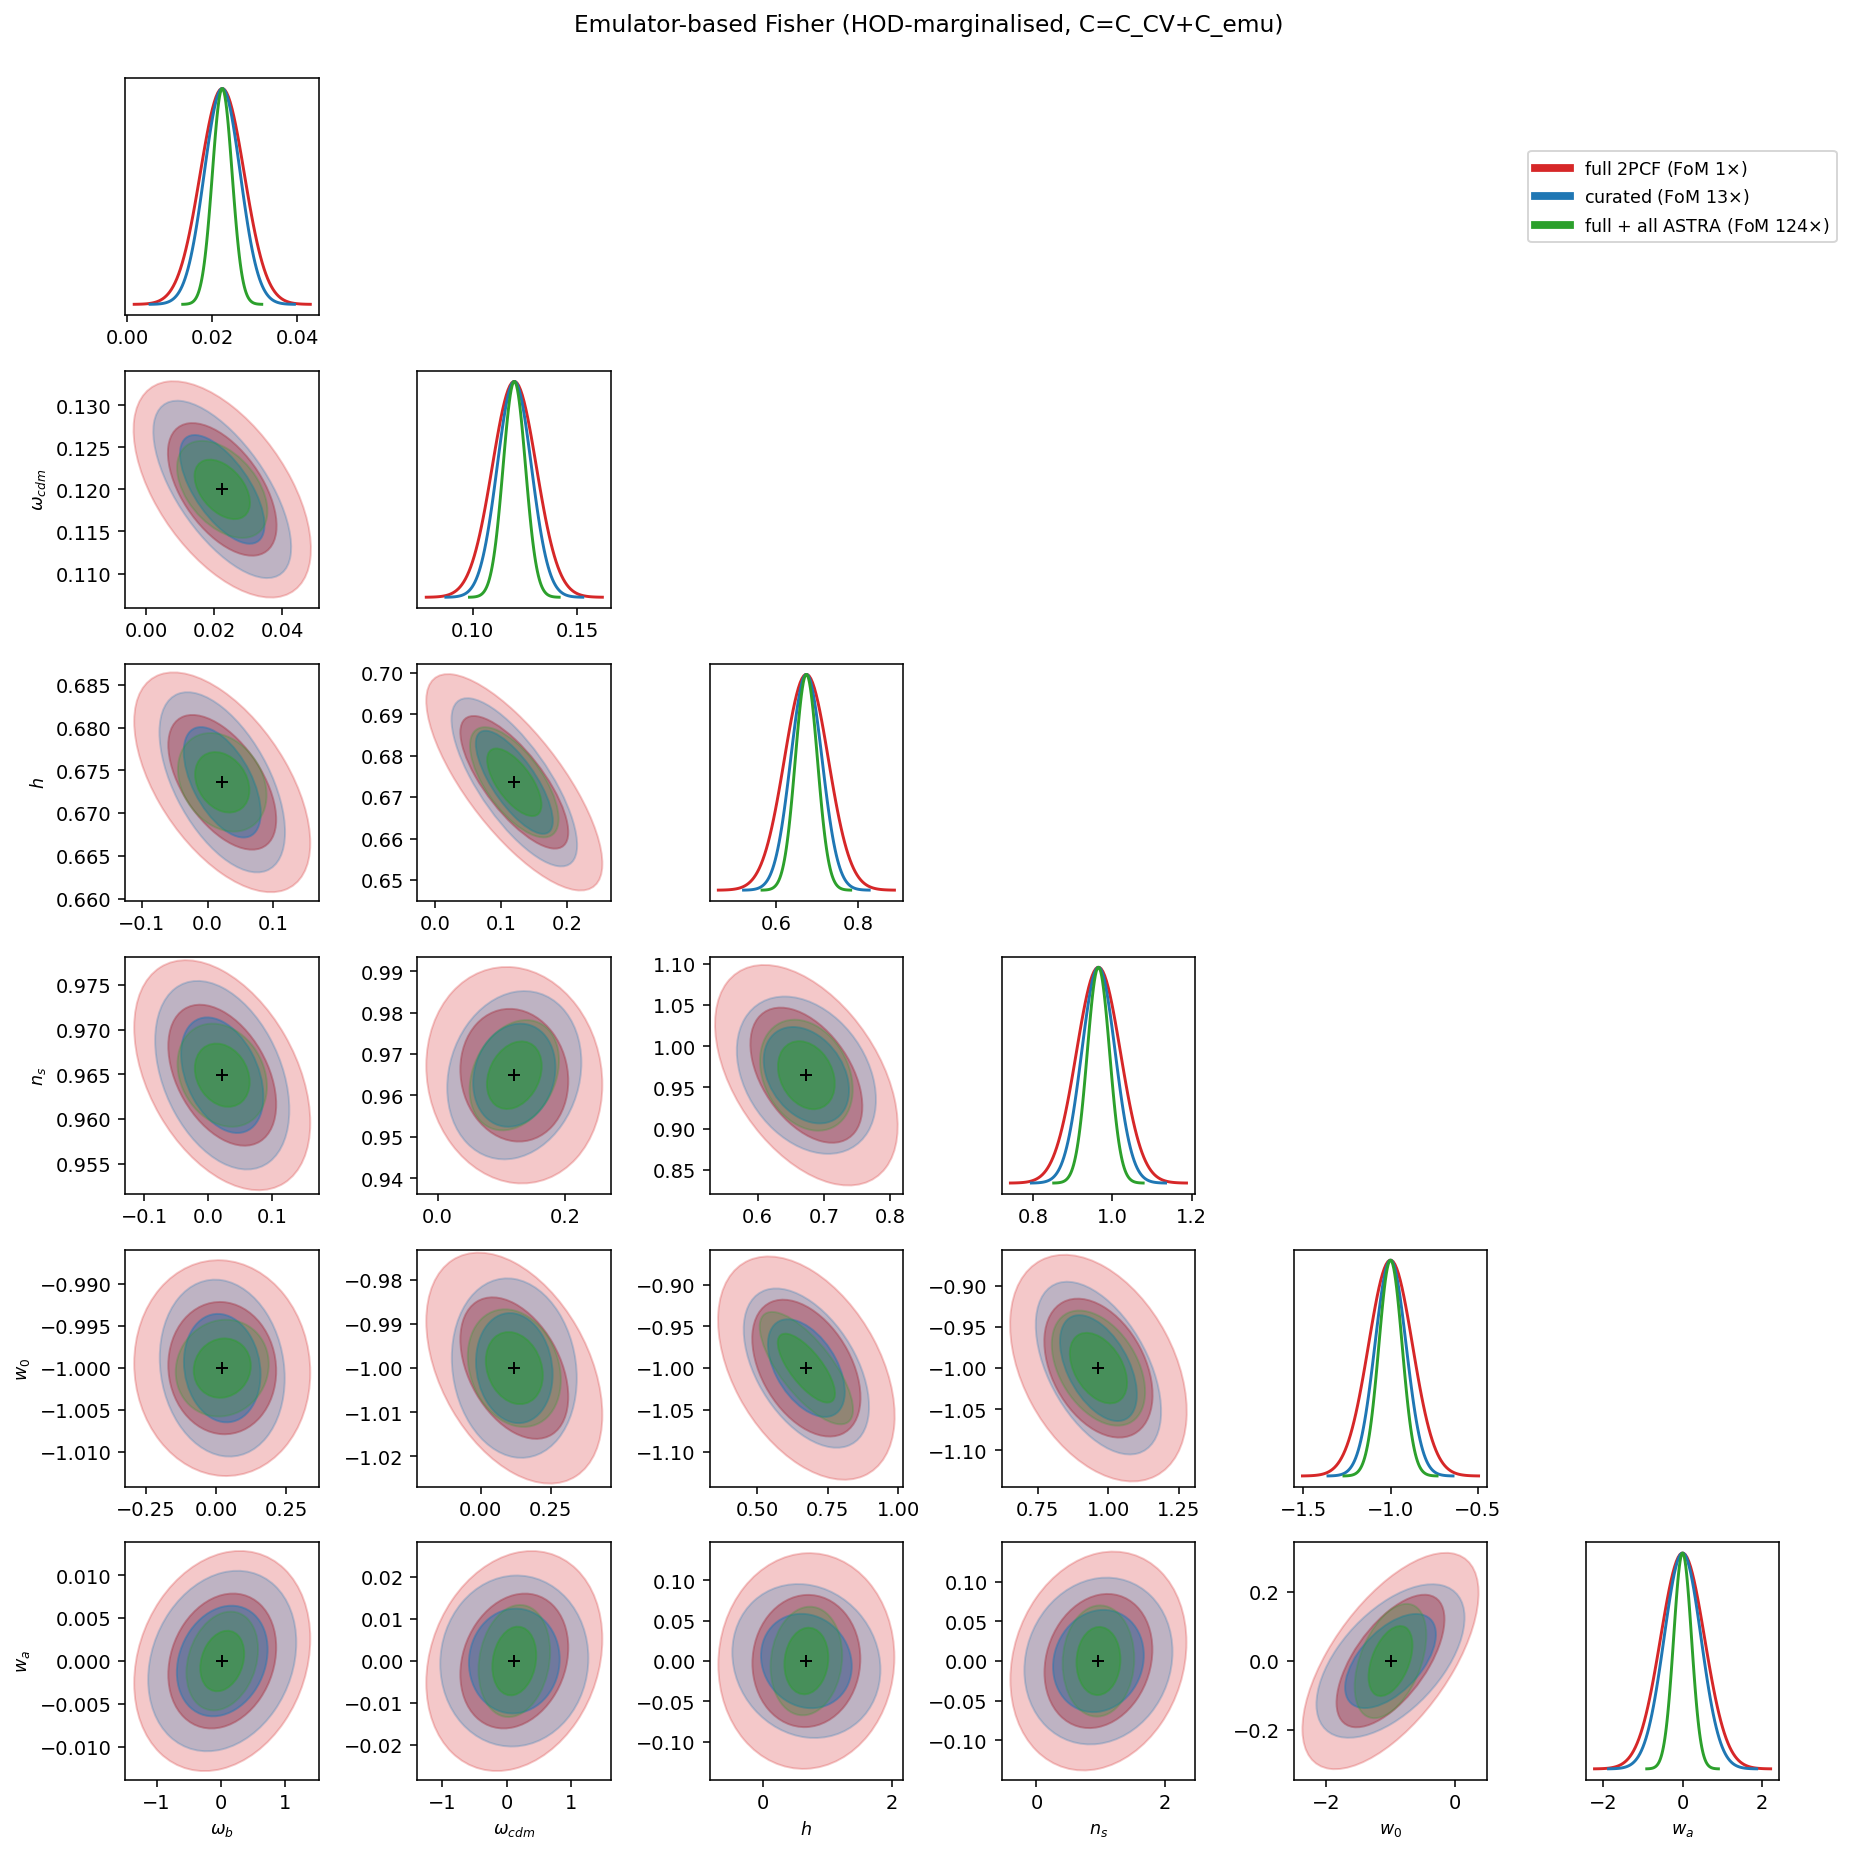
\includegraphics[width=0.8\textwidth]{emufisher_forecast.png}
\caption{HOD-marginalised corner for the three vectors (legend carries each FoM). The
curated and full$+$ASTRA ellipses are smaller \emph{and} rotated relative to the 2PCF.}
\label{fig:forecast}
\end{figure}

\subsection{Validation against the MCMC}
On the curated monopole vector with the 4 $\Lambda$CDM parameters, the Fisher $\sigma$ are
\textbf{$2.3$--$5.9\times$ looser than the MCMC} posteriors (ratios: $\omega_b$ 5.9,
$\omega_{\rm cdm}$ 3.5, $h$ 5.8, $n_s$ 2.3, HOD-marginalised; HOD-fixed is similar). The
Fisher is therefore \emph{conservative} in absolute terms here, while its \emph{relative}
predictions (the value-add ratios) match the MCMC value-add ($\times1.2$--$1.7$). The
absolute gap is consistent with a finite-difference derivative step that under-estimates
the local gradient and with the MCMC posterior being sharpened by the bounded prior and
the specific mock; it should be refined before quoting absolute $\sigma$, but does not
affect the leg-ranking or FoM \emph{comparisons}.

\subsection{Campaign forecast: FoM vs emulator error}
Scaling $\Cemu\!\to\!\alpha\Cemu$ traces what driving the emulator error down buys
(Fig.~\ref{fig:campaign}). The FoM is \textbf{steeply gated} by $\Cemu$:

\begin{center}\small
\begin{tabular}{lrrrrrrr}
\toprule
$\alpha$ & 1.0 & 0.5 & 0.3 & 0.1 & 0.03 & 0.01 & $\to0$ \\
median $\Cemu/\Ccv$ & 7.4 & 5.3 & 4.1 & 2.4 & 1.3 & 0.74 & 0 \\
FoM\,/\,FoM$(\alpha{=}1)$ & 1 & 4.7 & 13 & 97 & 610 & 2341 & $10^5$ \\
\bottomrule
\end{tabular}
\end{center}

Bringing the median environment-leg error to $\Cemu\!\approx\!\Ccv$ ($\alpha\!\sim\!0.03$)
already unlocks $\sim$$600\times$ FoM over the current emulator. This is the quantitative
campaign target: the value-add is realised only as $\Cemu$ falls below cosmic variance,
which (per the emulator note) is set by cosmology coverage.

\begin{figure}[h]\centering
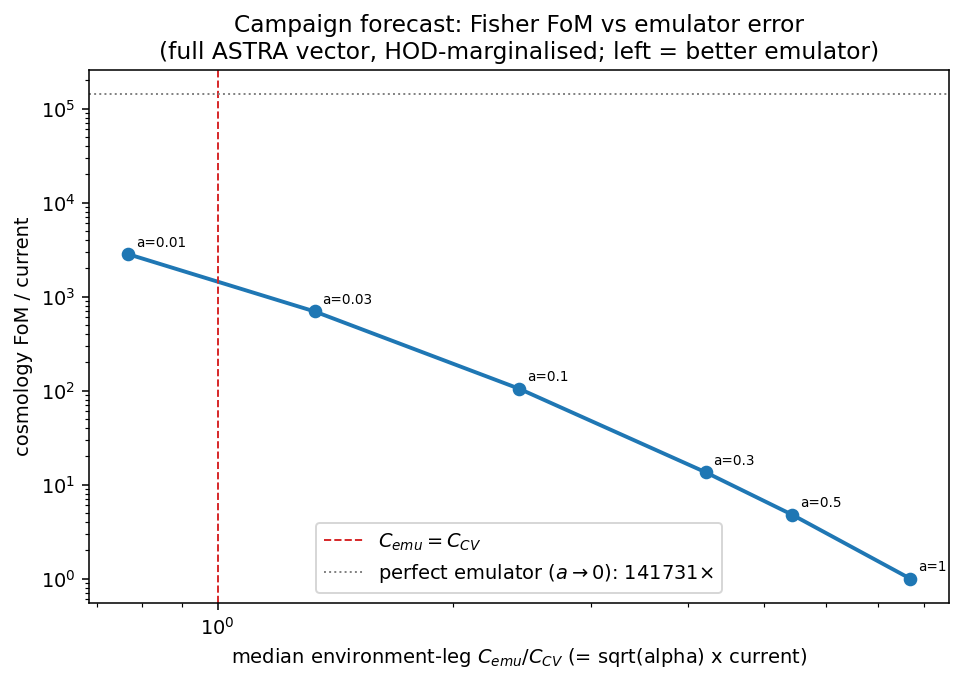
\includegraphics[width=0.7\textwidth]{emufisher_campaign.png}
\caption{Cosmology FoM vs the median environment-leg $\Cemu/\Ccv$ (full ASTRA vector,
HOD-marginalised). Left $=$ better emulator; the dashed line marks $\Cemu=\Ccv$.}
\label{fig:campaign}
\end{figure}

\section{Caveats}
The covariance is still the subbox estimate (no independent-mock suite under the
no-new-HOD constraint). Derivatives are at one fiducial ($c000$); the linear-Gaussian
Fisher is bounded by the MCMC validation (\S\,5). $C_{\rm emu}$ is from a single-phase
LOCO and is cosmology-averaged; a neighbourhood-matched $C_{\rm emu}$ would refine the
broad-prior numbers. $w_0,w_a$ rely on the quadrupole and remain the weakest directions.

\end{document}
